\title{Formulae for Oort Lore}
\author{Odradek}
\date{\today}

\documentclass[10pt]{article}

\pagestyle{headings}

\usepackage[margin=3cm]{geometry}
\usepackage[colorlinks=true, linkcolor=blue]{hyperref}
\usepackage{amsmath}
\usepackage{siunitx}
\usepackage{pgfplots}

\usetikzlibrary{intersections}

\makeatletter
\tikzset{%
	clear global paths/.style={
		execute at end picture=\clear@global@paths,
		name path global/.append code={
			\ifx\global@paths\pgfutil@empty
			\gdef\global@paths{##1}%
			\else
			\xdef\global@paths{\global@paths,##1}%
			\fi
		}
	},
	clear global paths now/.code={
		\expandafter\global\expandafter\let\csname tikz@intersect@path@name@#1\endcsname=\relax
	}
}
\let\global@paths=\pgfutil@empty
\def\clear@global@paths{%
	\edef\@temp{\noexpand\pgfkeys{/tikz/clear global paths now/.list={\global@paths}}}%
	\@temp
	\global\let\global@paths=\pgfutil@empty
	\global\let\tikz@intersect@namedpaths=\pgfutil@empty
}
\makeatother

\numberwithin{equation}{section}

\begin{document}
	\newcommand*{\ShowIntersection}[2]{
		\fill 
		[name intersections={of=#1 and #2, name=i, total=\t}] 
		[red, opacity=1, every node/.style={above left, black, opacity=1}] 
		\foreach \s in {1,...,\t}{(i-\s) circle (2pt)
			%node [above left] {\s}
			};
	}
	
	\maketitle
	\newpage
	
	\tableofcontents
	\newpage
	
	\begin{abstract}
		Some derivation for formulas that can be useful to calculate stuff in space.
	\end{abstract}
	
	\section{Conventions and Prerequisites}
	
	\subsection{Notation}
	
	\subsection{Variable Names}
	
	\begin{itemize}
		\item $s$: Distance
		\item $v_0$: Velocity at the beginning
		\item $v_{end}$: Velocity at the end
		\item $a$: Acceleration
		\item $a_{eff}$: Effective acceleration (any gravitational has been removed: $a_{eff} = a - g$)
	\end{itemize}
	
	When we need them in vector form, they are written as $\vec{s}$ for example.
	
	\subsection{Units}
	
	We are using either $km$ or $AU$ instead of $m$.
	
	\begin{itemize}
		\item $AU$: Astronomical Unit. $1 AU \approx$ \SI{149e+6}{\km}.
	\end{itemize}
	
	\subsection{Constants}
	
	\begin{itemize}
		\item $G \approx$ \SI{6.674e-18}{\N\km\squared\per\kg\squared}
	\end{itemize}
	
	\subsection{Setup of the Solar System}
	
	\begin{tabular}{l r r}
		Celestial Body & Distance [\unit{\astronomicalunit}] & Mass [\unit{\kg}]\\
		Sun & 0 & \\
		Mercury & 0.4 & \\
		Venus & 0.72 & \\
		Earth & 1 & \\
		Mars & 1.5 & \\
		Asteroid Belt & 2.2-2.3 & \\
		Jupiter & 5.2 & \\
		Saturn & 9.5 & \\
		Uranus & 19 & \\
		Neptune & 30.1 & \\
		Pluto & 39 & \\
		Kuiper Belt & 30-50 & \\
		Scattered Disc & 50-1000 & \\
		Oort Cloud & (2000-5000)-(\num{10000}-\num{100000}) & \\
	\end{tabular}
	
	\section{Travel Time Without Relativity}\label{TravelTime}
	
	\subsection{Constant Speed}
	
	From	
	\begin{equation}
		s = vt	\end{equation}	
	follows
	\begin{equation}
		t = s/v. \end{equation}
	
	\subsection{Under Acceleration}
	
	From	
	\begin{equation}
		s = 0.5at^2	\end{equation}
	follows	
	\begin{equation}
		t = \sqrt{2s/a}	\end{equation}	
	and a final velocity of	
	\begin{equation}
		v=at. \end{equation}
	
	\subsubsection{With Start Velocity}
	
	From	
	\begin{equation}
		s = v_0t + 0.5at^2 \end{equation}	
	follows	
	\begin{equation}\label{eq:1}
		t = \frac{-v_0 + \sqrt{v^2_0 + 2sa}}{a}	\end{equation}	
	and a final velocity of	
	\begin{equation}
		v_1 = v_0 + at.	\end{equation}	
	Note that the last formula can with the help of (\ref{eq:1}) also be written as	
	\begin{equation}
		v_1=v_0 + (-v_0 + \sqrt{v^2_0+2sa}) = \sqrt{v^2_0+2sa},	\end{equation}	
	from which we can get the final velocity without calculating the time first.
	
	\section{Agnus Journey Without Relativity}
	
	In our example we want to calculate the time and end velocity for the journey sections of the Agnus. We start escaping earth with four and two g at first, then take a trip to the asteroid belt with an acceleration and deceleration of one g, switching gears shortly after mars. We assume that Mars is currently located at a distance of $\SI{0.5}{\astronomicalunit} = \SI{74.8e+6}{\km}$.
	
	\paragraph{Phase one: First half of atmosphere.}
	we want to escape earth with an effective acceleration of $a_{eff1} = a-g = 4g = \SI{0.04}{\km\per\s\squared}$ until we reach a height of $s_1= \SI{5000}{\km}$, which is half of the exosphere. We just assume the computer keeps the effective acceleration at a constant $4g$.
	
	Then we reach the first destination after	
	\begin{equation}
		t_1 = \sqrt{2s_1/a_{eff1}} = \sqrt{\frac{\SI{10000}{km}}{\SI{0.04}{\km\per\s\squared}}} = \SI{500}{\s} = \SI{8.3}{\min}	\end{equation}	
	with a velocity of
	\begin{equation}
		v_1=a_{eff1}t_1=\SI{0.04}{\km\per\s\squared} \cdot \SI{500}{\s} = \SI{20}{\km\per\s}, \end{equation}	
	which will be our start speed for the next phase.
	
	\paragraph{Phase two: Second half of atmosphere.}
	Now we want to accelerate with a burn of $a_{eff2}=2g=\SI{0.02}{\km\per\s\squared}$ until we leave the exosphere. For this, we need to pass another $s_2=\SI{5000}{\km}$. Mind that we now have a non-zero start velocity of $v_1 = \SI{20}{\km\per\s}$.
	
	Then we reach the second destination after
	\begin{equation}
		t_2 = \frac{-v_1+\sqrt{v^2_1+2s_2a_{eff2}}}{a_{eff2}} = \frac {\SI{-20}{\km\per\s}+\sqrt{\SI{400}{\km\squared\per\s\squared}+\SI{200}{\km\squared\per\s\squared}}} {\SI{0.02}{\km\per\s\squared}}
		\approx \SI{224.7}{\s} \approx \SI{3.7}{\min} \end{equation}
	with a final velocity of
	\begin{equation}
		v_2 = v_1 + a_{eff_2}t_2
		= \SI{20}{\km\per\s} + \SI{0.02}{\km\per\s\squared} \cdot \SI{224.7}{\s}
		= \SI{24.5}{\km\per\s}. \end{equation}
	
	\paragraph{Phase three: Mars.}	
	Now we want to go to mars and have $s_3 = \SI{75e+6}{\km}, v_2 = \SI{24.5}{\km\per\s}$ and $a_{eff3} = \SI{0.01}{\km\per\s\squared}$.
	
	Let's calculate the final velocity first, this time. It is
	\begin{equation}
		v_3 = \sqrt{v^2_2 + 2s_3 a_{eff3}}
		= \sqrt{\SI{600}{\km\squared\per\s\squared} + \SI{1.5e+6}{\km\squared\per\s\squared}}
		= \SI{1225}{\km\per\s} \end{equation}
	which is about $0.3 \%$ of the speed of light and we expect not much relativistic effects here. With this, we can also calculate the travel time and get
	\begin{equation}
		t_3 = \frac{-v_2 + v_3}{a_{eff3}}
		= \frac{\SI{-24,5}{\km\per\s} + \SI{1224}{\km\per\s}}{\SI{0.01}{\km\per\s\squared}}
		= \SI{120049}{\s} = \SI{33.3}{\hour}. \end{equation}
	So a little more than thirty hours to get to mars this way. Nice!
	
	\paragraph{Phase four: To the asteroid belt.}
	
	We would like to have a velocity of $v_2 = \SI{24.5}{\km\per\s}$ again when we reach the asteroid belt in order to be slow down enough to dodge asteroids. To achieve this, we will further accelerate with $a_4 = 1 g$ for $s_4 = \SI{0.1}{\astronomicalunit}$ and then decelerate with $a_5 = -1 g$ for $s_5 = \SI{0.6}{\astronomicalunit}$.
	\begin{equation}
		v_4 = \sqrt{v^2_3 + 2s_4 a_4}
		= \sqrt{\SI{1500625}{\km\squared\per\s\squared} + \SI{300000}{\km\squared\per\s\squared}}
		= \SI{1342}{\km\per\s} \end{equation}
	\begin{equation}
		t_4 = \frac{-v_3 + v_4}{a_4}
		= \frac{\SI{-1225}{\km\per\s} + \SI{1342}{\km\per\s}}{\SI{0.01}{\km\per\s\squared}}
		= \SI{11687}{\s} = \SI{3.2}{\hour} \end{equation}
	\begin{equation}
		v_5 = \sqrt{v^2_4 + 2s_5 a_5}
		= \sqrt{\SI{1800964}{\km\squared\per\s\squared} - \SI{1800000}{\km\squared\per\s\squared}}
		= \SI{31}{\km\per\s} \end{equation}
	\begin{equation}
		t_5 = \frac{-v_4 + v_5}{a_5}
		= \frac{\SI{-1342}{\km\per\s} + \SI{31}{\km\per\s}}{\SI{-0.01}{\km\per\s\squared}}
		= \SI{131100}{\s} = \SI{36.4}{\hour} \end{equation}
	It can be assumed that the difference in the final velocity origins in rounding errors.
	
	\paragraph{Phase five: Through the asteroid belt.}
	
	Under the assumption that we did reach the final velocity of $v_2 = \SI{24.5}{\km\per\s}$ - which we will maintain - and that the asteroid belt spans $s_6 = \SI{0.1}{\astronomicalunit}$, the passage takes
	\begin{equation}
		t_6 = s_6 / v_2 = \frac{\SI{15e+6}{\km}}{\SI{24.5}{\km\per\s}} = \SI{612e+3}{\s}
		= \SI{170}{\hour}. \end{equation}
	That takes way to long, so let's add an acceleration of 1 g to that:	
	\begin{equation}
		v_6 = \sqrt{v^2_2 + 2s_6 a_4}
		= \sqrt{\SI{600}{\km\squared\per\s\squared} + \SI{300000}{\km\squared\per\s\squared}}
		= \SI{548}{\km\per\s} \end{equation}
	\begin{equation}
		t_6 = \frac{-v_2 + v_6}{a_4}
		= \frac{\SI{-24.5}{\km\per\s} + \SI{548}{\km\per\s}}{\SI{0.01}{\km\per\s\squared}}
		= \SI{52350}{\s} = \SI{14.5}{\hour} \end{equation}
	Now that looks better.
	
	\paragraph{Phase six: Out to oort.}
	
	Constant acceleration of $1 g$ is kept. We want to have a nice chart, in which we can see when we arrive at which planet's orbit. This is delivered by the function
	\begin{equation} \begin{aligned}
		s(t) & = s_0 + v_6 t + \frac{1}{2} g t^2
		= \SI{330e+6}{\km} + \SI{548}{\km\per\s} t + \SI{0.01}{\km\per\s\squared} t^2 \\
		& = \SI{2.2}{\astronomicalunit} + \SI{13.152e-3}{\astronomicalunit\per\hour} t
			+ \SI{864e-6}{\astronomicalunit\per\hour\squared} t^2, \end{aligned} \end{equation}
	where we have switched the units from $km$ and $s$ to $au$ and $h$.
	
	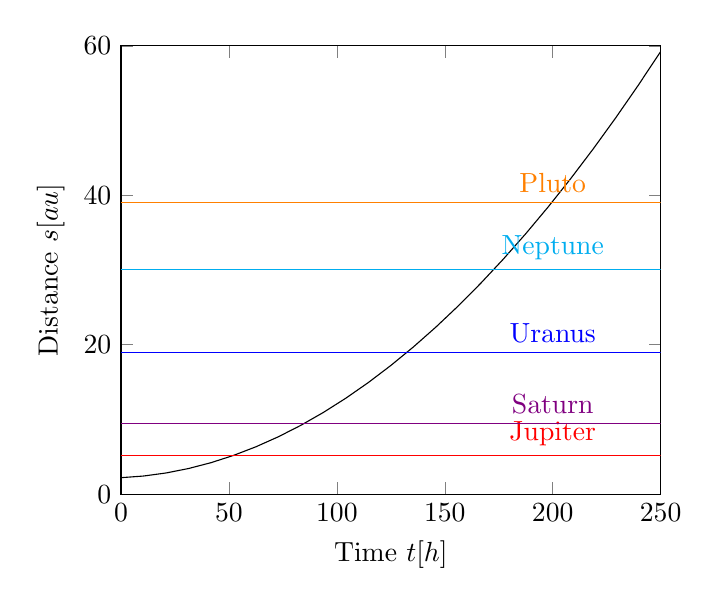
\begin{tikzpicture}[clear global paths]
		\begin{axis}[
			xlabel={Time $t[h]$},
			ylabel={Distance $s[au]$},
			xmin = 0,
			xmax = 250,
			ymin = 0,
			ymax = 60]
			
			\addplot [name path global=leavingTrajectoryClose, domain=0:250] {2.2 + 0.012152*x + 0.000864*x^2};			
			\addplot [name path global=jupiterOrbit, domain=0:250, color=red] {5.2} node[above,pos=0.8] {Jupiter};
			\addplot [name path global=saturnOrbit, domain=0:250, color=violet] {9.5} node[above,pos=0.8] {Saturn};
			\addplot [name path global=uranusOrbit, domain=0:250, color=blue] {19} node[above,pos=0.8] {Uranus};
			\addplot [name path global=neptuneOrbit, domain=0:250, color=cyan] {30.1} node[above,pos=0.8] {Neptune};
			\addplot [name path global=plutoOrbit, domain=0:250, color=orange] {39} node[above,pos=0.8] {Pluto};
			\fill [name path global=kuiperBelt, fill=green, nearly transparent] (0,500) -- (250,500) -- (250,300) -- (0,300) node[above,pos=0.8] {Kuiper Belt};
			
			\ShowIntersection{leavingTrajectoryClose}{jupiterOrbit}
			\ShowIntersection{leavingTrajectoryClose}{saturnOrbit}
			\ShowIntersection{leavingTrajectoryClose}{uranusOrbit}
			\ShowIntersection{leavingTrajectoryClose}{neptuneOrbit}
			\ShowIntersection{leavingTrajectoryClose}{plutoOrbit}
			\ShowIntersection{leavingTrajectoryClose}{kuiperBelt}
		\end{axis}
	\end{tikzpicture}
	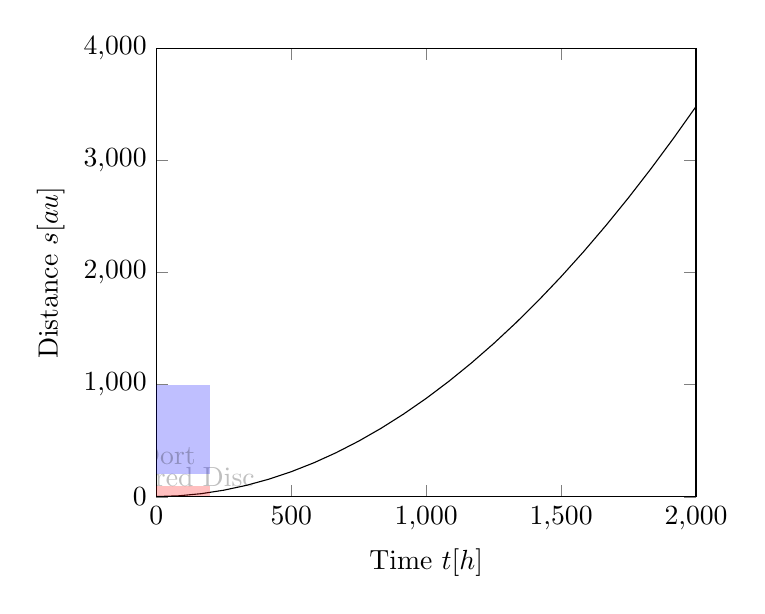
\begin{tikzpicture}[clear global paths]
		\begin{axis}[
			xlabel={Time $t[h]$},
			ylabel={Distance $s[au]$},
			xmin = 0,
			xmax = 2000,
			ymin = 0,
			ymax = 4000]
			
			\addplot [name path global=leavingTrajectoryDistant, domain=0:2000] {2.2 + 0.012152*x + 0.000864*x^2};
			\fill [name path global=scatteredDisc, fill=red, nearly transparent] (0,100) -- (200,100) -- (200,5) -- (0,5) node[above,pos=0.8] {Scattered Disc};
			\fill [name path global=Oort, fill=blue, nearly transparent] (0,1000) -- (200,1000) -- (200,200) -- (0,200)node[above,pos=0.8] {Oort};
			
			\ShowIntersection{leavingTrajectoryDistant}{scatteredDisc}
			\ShowIntersection{leavingTrajectoryDistant}{Oort}
		\end{axis}
	\end{tikzpicture}
	
	Oort cloud is reached after about $66$ days since leaving earth with a velocity of
	\begin{equation} \begin{aligned}
		v_{oort} & = \sqrt{v^2_6 + 2s_{oort} g}
		= \sqrt{\SI{13.152e-3}{\astronomicalunit\per\hour} + 2 \cdot \SI{197.8}{\astronomicalunit}\SI{864e-6}{\astronomicalunit\per\hour\squared}} \\
		& = \SI{596e-3}{\astronomicalunit\per\hour} = \SI{24824}{\km\per\s}, \end{aligned} \end{equation}
	which is about $8\%$ of the speed of light.
	
	\section{Travel Time With Special Relativity}
	
	\section{Constant Speed}
\end{document}